\section{Introduction}
\label{socksdirect:sec:intro}

The theme of this chapter is the acceleration of operating system communication primitives, as shown in Figure \ref{socksdirect:fig:sys-arch}.

\begin{figure}[htbp]
	\centering
	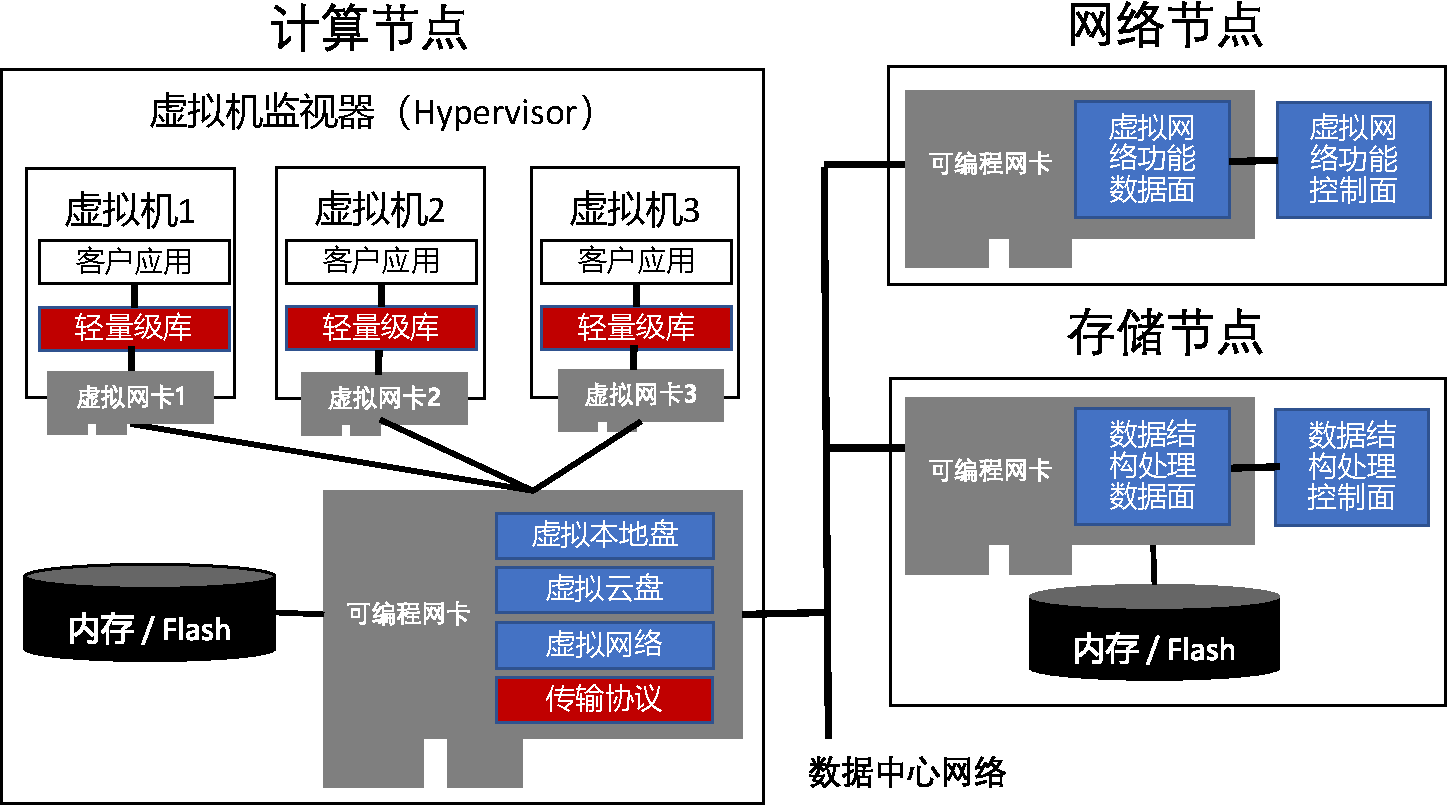
\includegraphics[width=0.8\textwidth]{images/sys_arch.pdf}
	\caption{The theme of this chapter: acceleration of operating system communication primitives, marked with a bold italic line background.}
	\label{socksdirect:fig:sys-arch}
\end{figure}

As the last research work introduced in this paper, we have implemented a user-space socket communication library that is compatible with existing applications, using shared memory and RDMA as the communication methods between processes on the same machine and between different hosts, respectively. As a supplement, based on the ClickNP programming framework and KV-Direct data structure processing service proposed in previous chapters, we have implemented a scalable RDMA connection number in the programmable network card.

\begin{figure}[htbp]
	\centering
	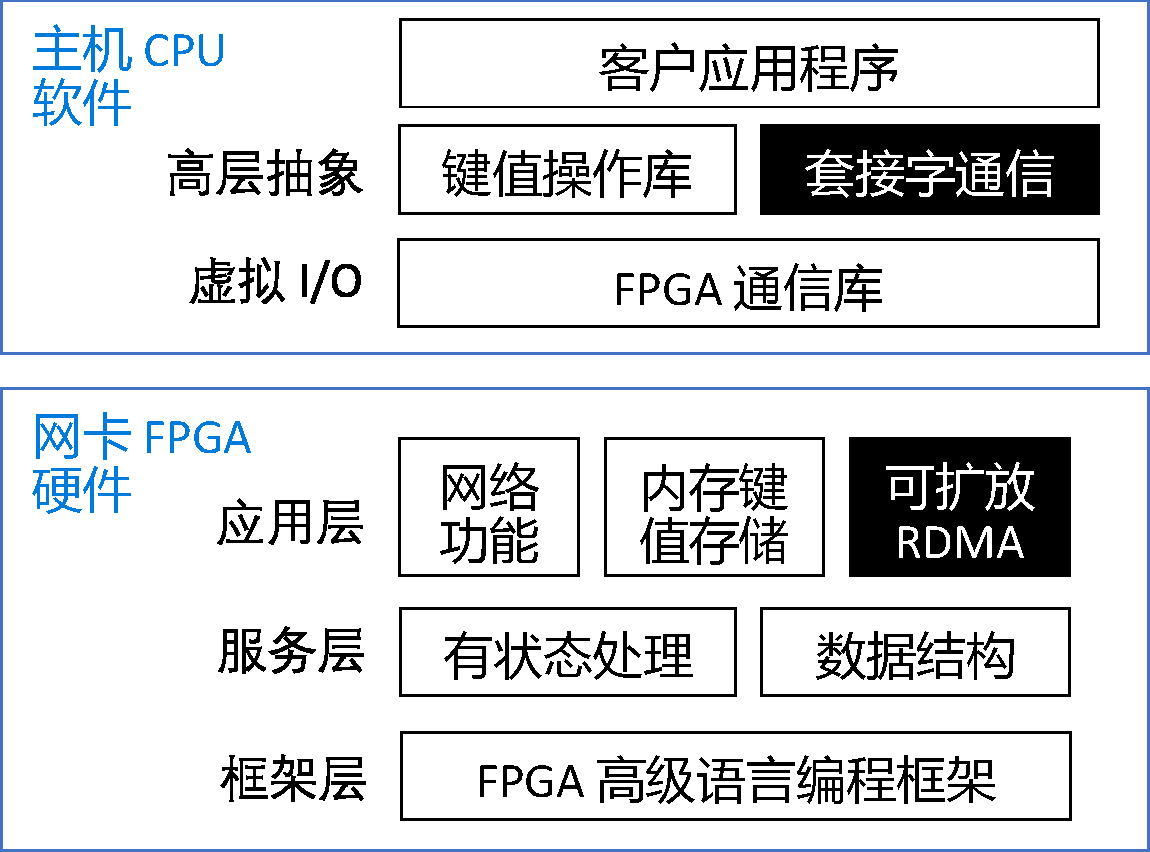
\includegraphics[width=0.5\textwidth]{images/sw_hw_codesign.pdf}
	\caption{The position of this chapter in the programmable network card software and hardware architecture.}
	\label{socksdirect:fig:sw-hw-codesign}
\end{figure}

%Most cloud applications use the socket API for inter-process communication among components or containers inside a same server and across data center network, in addition to serving Internet users. For example, communication intensive applications (\textit{e.g.} Nginx and memcached) spend 50\%$\sim$90\% of CPU time in the OS kernel, mostly processing socket operations.
%The overhead of Linux socket attributes to kernel crossing in system calls, context switch, process scheduling, synchronization, memory copy, cache miss and TCP transport.
%Applications in high performance computing have a long tradition of using shared memory for intra-server communication and RDMA for inter-server, thus avoiding the overheads above.
%However, these abstractions are radically different from socket, so it is complicated and potentially insecure to port socket applications to shared memory and RDMA.
%The overhead of Linux socket becomes salient given the rapid growth of network speed and number of CPU cores per server. %We benchmark communication intensive applications (\textit{e.g.} Nginx and memcached) and find that 50\%$\sim$90\% of CPU time is spent in the OS kernel. When more CPU cores are utilized, they even spend a larger portion of time in the kernel~\cite{boyd2010analysis}. In addition to CPU overhead, latency is also a problem. The round-trip time (RTT) between two processes communicating with shared memory can be as low as 0.2$\mu$s, while TCP socket RTT between two cores is $\approx$16$\mu$s. In a data center, the RTT between RDMA servers is also one order of magnitude lower than kernel TCP/IP stack.

The Socket API is the most widely used communication primitive in modern applications, typically used for communication between processes, containers, and hosts. 
Linux sockets can only achieve latency and throughput that are one to two orders of magnitude worse than bare hardware (such as shared memory and RDMA).
In recent years, a lot of work has been aimed at improving socket performance. 
Existing methods either optimize the kernel network protocol stack \cite {lin2016scalable,han2012megapipe,yasukata2016stackmap}, move the TCP/IP protocol stack to user space \cite {jeong2014mtcp,marinos2014network,seastar,fstack,libvma}, or offload the transport layer to RDMA network cards \cite{rsockets,socketsdirect}.
However, all these solutions have limitations in terms of compatibility and performance. 
Most of them are not fully compatible with Linux sockets in aspects such as process fork, event polling, multi-application socket sharing, and intra-host communication. 
Some of them \cite {jeong2014mtcp} have isolation issues, not allowing multiple applications to share a network card. 
Despite these efforts to improve performance, there is still a lot of room for performance improvement. Existing work cannot achieve performance close to bare RDMA and shared memory because they cannot eliminate important overheads such as multi-thread synchronization, buffer management, and memory copying. 
For example, sockets are shared among multiple threads within a process, so many systems use locks to avoid race conditions.

%For inter-server communication, most works leverage a user-space stack~\cite{dunkels2001design,jeong2014mtcp,libvma,openonload} to achieve kernel bypass, but the CPU still needs to handle reliable transport. As RDMA becomes widely available in data centers, we hope to offload the transport to RDMA network cards when the peer supports RDMA. Furthermore, most works assume only one connection per pair of processes. However, load balancers, web servers and application gateways serve many concurrent connections~\cite{nishtala2013scaling,lin2016scalable,belay2017ix}. In light of this, both connection setup, event notification and data transmission under high concurrency need to be efficient.

%To demonstrate high performance, most existing works propose new abstractions for inter-process and inter-server communication.  existing socket applications need modifications to use the new abstractions. Furthermore, these stacks are not optimized for a large number of concurrent or short-lived connections, which is an important workload to serve Internet users and large distributed systems.

%One line of research optimize the kernel code or design user-space compatible stacks for higher socket performance. The kernel optimization approach does not eliminate context switch overhead, while system call batching introduces extra latency. User-space stacks are mostly designed for inter-server connections. With the trend of containerized micro-services, we expect an increasing number of applications or containers to be hosted on each server, where inter-process communication (IPC) inside server has more significance.

%To simplify deployment, we hope to accelerate existing applications without modification to the code. \textit{Socket compatibility} adds another dimension of challenge. The socket interface was designed for networking and IPC in millisecond scale, when memory copy, context switch, synchronization, cache miss and cache migration were considered inexpensive~\cite{barroso2017attack,belay2017ix}. An efficient socket architecture for microsecond-scale networking and IPC requires minimizing all overheads above. The semantics lead to challenges. First, the send buffer can be modified by application after non-blocking \texttt{send}, and the receive buffer is not determined until application calls \texttt{recv}. Data copy on \texttt{send} and \texttt{recv} seems mandatory. Second, connections are shared by processes and threads after \texttt{fork} and thread creation. It is challenging to avoid synchronization in this multi-producer and multi-consumer FIFO model. Third, multiple processes listening on a same IP and port compete for incoming connections.

Recognizing these limitations, this chapter designs \sys{}, a user-space socket system that achieves compatibility, isolation, and high performance simultaneously.
\begin{ecompact}
\item \textbf {Compatibility}.
Applications can use \sys{} as a substitute for Linux sockets without any modifications.
\sys{} supports both intra-host and inter-host communication, and behaves correctly during process forks and thread creation.
If the remote endpoint does not support \sys{}, the system will transparently fall back to standard TCP.
\item \textbf {Isolation}.
Firstly, \sys{} maintains isolation between applications and containers, i.e., no application can listen to or interfere with connections between other applications, and a malicious program cannot cause erroneous behavior at its connection endpoint.
Secondly, \sys{} can enforce access control policies to prevent unauthorized connections.
\item \textbf {High performance}.
\sys{} provides high throughput and low latency, comparable to raw RDMA and shared memory, and can achieve performance scaling across multiple CPU cores.
\end{ecompact}

To achieve high performance, \sys{} fully utilizes the capabilities of modern hardware. It uses RDMA for inter-host communication and \emph {shared memory} for intra-host communication. However, converting socket operations into RDMA and shared memory operations is not straightforward.
Simple solutions may violate compatibility or leave a lot of performance on the table.
For example, after a socket \textbf {send()} returns, the application may overwrite the buffer.
However, RDMA send operations require write-protecting the buffer.
Existing work \cite {rsockets} either provides a zero-copy API that is incompatible with unmodified applications, or requires the protocol stack to manage internal buffers and copy data from the buffer.
%For example, \textcolor{red}{Take socket send() to RDMA send operations as an example here. If no memory copy, compatibility. If memory copy, performance degradation. Btw, how to point out isolation problem here?}

To achieve all three goals simultaneously, it is first necessary to understand how Linux sockets provide compatibility and isolation. Linux sockets provide a Virtual File System (VFS) abstraction to applications. Through this abstraction, application developers can communicate like operating files without delving into the details of network protocols. This abstraction also provides good isolation between applications sharing address and port spaces. However, the VFS abstraction is very complex, and many APIs are inherently unscalable \cite {clark1989analysis,boyd2010analysis,jeong2014mtcp}.

Despite the universality and complexity of VFS, many commonly used socket operations are actually quite simple. Therefore, the design principle of this chapter is to optimize for common cases while maintaining compatibility.

To accelerate data transmission while maintaining isolation in connection management, \sys{} separates the control and data planes \cite {peter2016arrakis}.
In each host, a \emph {monitor} daemon is introduced as the \emph {control plane} to enforce access control policies, manage address and port resources, dispatch new connections, and establish transport channels between communication endpoints.
The \emph {data plane} is handled by a dynamically loaded user-space library \libipc{}, which intercepts function calls to the standard Linux C library. \libipc{} implements the socket API in user space and forwards non-socket related APIs to the kernel.
Applications can take advantage of \libipc{} by loading the library using the \emph {LD\_PRELOAD} environment variable in Linux.

In \sys{}, data transmission and event polling are handled directly between peer processes, while connection establishment is delegated to the monitor.
This chapter utilizes various techniques to efficiently use hardware and improve system efficiency.
Typically, socket connections are shared between threads and processes created by fork.
To avoid race conditions when accessing socket metadata and buffers, synchronization is needed.
By using a token-based sharing method instead of locking for each operation, \sys{} eliminates synchronization overhead in common cases.
When sending and receiving data from the network card, existing systems allocate buffers for each packet.
To eliminate buffer management overhead, this chapter designs a ring buffer exclusive to each connection, with a copy at both the sender and receiver, and then synchronizes from the sender's ring buffer to the receiver's using RDMA and shared memory.
To achieve zero-copy for larger messages, \sys{} remaps pages using the virtual memory mechanism.
%Finally, we observe that cooperative context switch is faster than process wakeup, so we design a mechanism to allow CPU time sharing among polling processes.

The design of \sys{} presents numerous challenges. 
(1) How can a socket be shared among threads and forked processes without locking?
(2) How can it scale to accommodate many concurrent connections?
(3) How can shared memory and RDMA be utilized efficiently for intra- and inter-host communication?

In both multi-thread and multi-process scenarios, a connection may be shared by multiple senders and receivers.
Existing approaches require locking to protect shared queue and metadata.
To avoid the overhead of locking, we treat each thread as a separate process.
%, even if the threads have shared memory address space.
\libipc{} uses thread-specific storage and creates peer-to-peer queues between each pair of communicating threads.
To preserve FIFO semantics, we optimize for the common case while preparing for the worst case, and take special care on fork and thread creation.

To efficiently handle many concurrent connections, we need to save memory footprint and improve spatial locality.
For each pair of threads, \sys multiplexes socket connections through one message queue.
Instead of maintaining a separate buffer for each connection and an event notification queue, we receive events and data from the message queue directly.
Observing the event-driven behavior of applications, in normal case the data in queue is fetched by the application in send order.
We design carefully to enable fetching from the middle of queue and solve the head-of-line blocking problem.

We leverage different transports to push performance to the limits of underlying hardware.
For inter-process and inter-container sockets within a same host, we use shared memory in user space.
For sockets among hosts in an RDMA enabled data center, \sys can transparently determine whether the remote endpoint supports \sys.
we fall back to kernel TCP socket.
We design different queue structures for shared memory and RDMA.
We use batched one-sided RDMA write and amortize polling overhead with shared CQ.
%In \sys, sending a small message involves only one cache migration or one-sided RDMA write.
To remove memory copy for large messages, we use \emph{page remapping} to achieve transparent zero copy.
To share a CPU core efficiently among multiple active threads, \sys uses \emph{cooperative multitasking} to remove thread wakeup overhead.

\fi

%The POSIX socket API was designed for networking and IPC in millisecond scale, leading to two performance challenges. First, connections are shared by processes and threads after \texttt{fork} and thread creation. Linux protects this multi-producer multi-consumer FIFO with locks. To scale a shared socket, we \textit{optimize for the common case and prepare for the worst case}. Senders transmit data via different queues in parallel. To ensure receiver ordering, based on the observation that applications seldom receive concurrently from a shared socket, the sender designates a receiver with exclusive access. We further develop mechanisms to avoid deadlock and starvation, in addition to handling unconsumed buffers during \texttt{fork} and thread creation.

%Second, the send buffer can be modified by application after \texttt{send}, and the receive buffer is not determined until application calls \texttt{recv}. Data copy on \texttt{send} and \texttt{recv} seems mandatory. To avoid memory copy of large buffers, we extend the \textit{page remapping} approach~\cite{thadani1995efficient,chu1996zero}, which enables copy-on-write upon \texttt{send} and remaps send buffer to receiver's virtual address upon \texttt{recv}.
%First, we intercept \texttt{memcpy} of full pages to reduce copy-on-write. Second, we move kernel-based page allocation to user-space while preserving security.
%As a result, we achieve zero copy for both shared memory, RDMA and TCP transport.

\sys {} achieves latency and throughput close to the performance of underlying shared memory queues and bare RDMA.
In terms of latency, \sys {} achieves 0.3 microseconds RTT for intra-host sockets, which is 1/35 of Linux, and only 0.05 microseconds higher than bare-metal shared memory queues. For inter-host sockets, \sys {} achieves 1.7 microseconds RTT between RDMA hosts, almost the same as bare RDMA writes, and 1/17 of Linux.
In terms of throughput, a single thread can send 23~M intra-host messages per second (20 times of Linux) or 18~M inter-host (15 times of Linux, 1.4 times of bare RDMA writes).
For large messages, through zero-copy, a single connection can saturate the bandwidth of a 100 Gbps network card.
The above performance can be linearly scaled with the number of cores.
\sys {} provides significant acceleration for actual applications.
For example, the HTTP request latency of Nginx~\cite{nginx} is reduced to 1/5.5, and the latency of the standard RPC library can also be reduced by 50%.

In summary, this chapter makes the following contributions:
\begin{ecompact}
\item Analyzes the overhead of Linux sockets.
\item Designs and implements \sys {}, a high-performance user-space socket system that is compatible with Linux and can maintain isolation between applications.
\item Supports technologies such as fork, lock-free connection sharing, ring buffer, and zero-copy, which may be useful in many scenarios beyond sockets.
\item Evaluations show that \sys {} can achieve performance comparable to RDMA and shared memory queues.
\end{ecompact}

We evaluate the end-to-end performance of \sys{} using two categories of applications: \textit{network functions} and \textit{web services}. For a multi-core pipelined network function (NF) chain, a socket application achieves comparable performance with a state-of-the-art NF framework~\cite{panda2016netbricks}. We also evaluate \sys{} on a standard web application composed of a load balancer, a web service, and a key-value store. For an HTTP request that involves multi-round-trip key-value store accesses, \sys{} reduces end-to-end latency by two-thirds.

\iffalse
This paper makes the following contributions:
\begin{ecompact}
	\item A Linux compatible, secure, and high-performance user-space socket system that supports both inter-process, inter-container, and inter-host communication.
	\item A per-host monitor daemon for trusted control plane and peer-to-peer queues for a scalable data plane.
	\item A multi-sender and multi-receiver lockless queue to fully support fork and multi-thread socket sharing.
	\item A memory-efficient message queue that multiplexes multiple sockets and allows fetching from any socket, while using shared memory and RDMA transports efficiently.
\end{ecompact}
\fi
